\documentclass[final]{cmpreport}

\usepackage{enumitem}
\usepackage{wasysym}
\usepackage{framed}
\usepackage{pgfgantt,rotating}
\usepackage{subfloat}
\usepackage{listings}
\usepackage{xcolor}
\usepackage{colortbl}
\usepackage{url}
\usepackage{hyperref}

\title{An Evaluation of HTML5\\as a Mobile Gaming Platform}

\author{Joshua Barnett}

\registration{5939968}
\supervisor{Professor Andy Day}

\ccode{CMPC3P2Y}

\summary{
This is my abstract.
}

\acknowledgements{
These are my achknowledgements.
}

\begin{document}

\section{Introduction}
For the past five years, it has become evident that mobile devices have risen as one of the foremost ways in which the modern world consumes media and entertainment. Alongside this, a new web standard has been developing: HTML5. HTML5 (HyperText Markup Language), a popularly abused buzzword, represents a new language specification with the primary purpose of succeeding where its predecessors failed, in delivering rich interactive content. ``HTML5'' has become an all encompassing term that includes a host of technologies, because this language alone cannot fully deliver rich web experiences. Technologies such as JavaScript (JS), Cascading Style Sheets (CSS), Scalable Vector Graphics (SVG), the Document Object Model (DOM) and WebGL have also been playing an integral part in shaping the modern web landscape. When used together in various combinations, these form a Web Platform\footnotemark[1] on which to convey content and information in new and interesting ways. It is currently the convention to refer to this new platform as solely HTML5 because this is where all these technologies stem from.

\footnotetext[1]{\url{http://docs.webplatform.org/wiki/Main_Page}}

``Linux'' has similarly been distorted as an umbrella term for Linux based operating systems such as Debian, Fedora, and Ubuntu. Nevertheless, ``Linux'' alone is just the open-source kernel which lies at the heart of these distributions which on its own would not be of much use.

Original equipment manufacturers (OEMs) such as Apple, LG, Nokia and Samsung are becoming progressively competitive in producing better mobile devices for the global market. They offer higher resolution displays, more memory capacity, and increasingly faster processors. This escalation in performance has been a key instigator in the growing support and optimization of HTML5 delivery on mobiles. However, it has only just begun to reach the requirements needed for delivering interactive real-time graphics applications such as video games.

\subsection{Project Goals}
The purpose of this project is to evaluate the current state of HTML5 and its companion technologies on the mobile platform, while assessing if they provide a suitable means to develop and deploy games. To assist my research I will be designing and creating my own game, expanding my personal understanding of the platform along the way. During the early years of my education, I taught myself how to draw and animate in Adobe Flash through watching online tutorials. I then learnt ActionScript and used this new skill to make games that were sold for sponsorship on various Flash gaming portals. However, since that time the industry has been shifting away from using third-party proprietary plugins in favour of open technologies such as HTML5. I feel this project will encourage me to research and learn these emerging technologies and the knowledge gained will provide me with a strong foundation for a career in industry.

\section{HTML5}
HTML5 is the fifth iteration of the hypertext mark up language. During its previous iterations such as HTML 4.01 and XHTML 1.1 there was minimal support for multimedia content. This resulted in a void that was promptly filled by third-party plugins such as Adobe Flash and Microsoft Silverlight. Such plugins allowed for easy presentation of media such as video, audio and even allowed for interactivity that was used to great effect in games.

Unfortunately many of these plugins are proprietary and closed-source which prevents developers from fixing and debugging inherent issues in the technology. Instead they are dependant on the technology owner for solutions while being limited to reporting them or finding ``temporary'' workarounds. Plugins often require some form of installation process as they are ``add-ons'' and exist outside of scope of the \textit{W3C} standards.

\citet{Jobs} famously professed his concerns about Flash and presented sound reasoning as to why Apple had no intentions of supporting or integrating Flash into their \textit{iOS} devices. Flash was also briefly available for Android but was short lived and eventually discontinued by Adobe. Adobe is continuing to making strides into the mobile platform with their new runtime AIR\footnotemark[2]. HTML5 is still currently a work in progress but the \cite{W3C} have made plans to stabilize the specification and help it reach \textit{Recommendation\footnotemark[3]} status as of this year.

\footnotetext[2]{\url{https://www.adobe.com/aboutadobe/pressroom/pressreleases/201002/021510FlashPlayerMWC.html}}
\footnotetext[3]{\url{http://www.w3.org/2005/10/Process-20051014/tr.html\#rec-publication}}

\subsection{The Document Object Model (DOM)}
The DOM is the core of what drives modern web applications. It provides a means to manipulate the structure and style of the original document loaded from a web server at run-time on the client side.

What makes HTML different from most compiled languages such as \textit{C++} and \textit{Java}, is its a interpreted language. Compiled languages are typically converted into a binary format that compresses their instructions into machine-code allowing for quicker execution. Interpreted languages such as Python and Ruby in contrast are often read line-by-line with their instructions parsed and executed at run-time.

When HTML is interpreted by a web browsers it is parsed into a DOM. The DOM is essentially a representation in memory of what was originally marked down in the static HTML document. This allows the browsers to interpret relations between elements and use them to render the document appropriately. While in memory the information is not longer static allowing for manipulation by other technologies such as JS.

One example of where this manipulation is used to great effect is the SPA (single-page application). SPAs have significant advantages over that of traditional websites as they can provide a seamless user experience similar to that of desktop applications. Instead of navigating through links that loading separate HTML pages they use states to manage the flow, loading information dynamically when required or requested. This technique shrinks factors such as load times, enables rich interactions, and responsiveness while encouraging reuse. \citep{Takada}

\subsection{Web Browsers}
Web browsers are client side applications that render the information requested by the user and then sent from a web server. Many of the popular browser vendors such as Google (Chrome), Apple (Safari), and Mozilla (Firefox) all have a mobile counterpart. However these mobile counterparts often support a subset of features in their desktop editions making much of the fringe HTML5 features even less accessible.

\subsection{Cross Compatibility}
Getting a single web application to render and function consistently across a range of browsers can be a huge undertaking. This task has grown exponentially with the introduction of mobile devices and their endless combinations of hardware, operating systems, and mobile browser applications. Each combination of these variables has the potential to produce unique bugs and quirks specific to a particular test case. As the specification of HTML5 was being developed much of the new features have been implemented in browsers at the discretion of the vendor. This has quickly led to cross compatibility issues as older browsers will support less of these new features and not necessarily be consistent with the other browsers that were available at the time.

Depending on the project specification a developer can rapidly become limited by what features of HTML5 they can utilise. For instance one such feature I had planned on using when initially developing my mobile game was \textit{viewport units}. This feature allows for the scaling of elements based upon the current viewport's dimensions which is especially useful on mobile devices for scaling visual elements relative to the screen's aspect ratio and pixel density. However the stock web browsers on mobile devices have only recently added support for this feature with it being introduced in version 4.4 of Android and 6.0 of iOS.

\begin{figure}[h]{A compatibility table for viewport units \label{viewport}}
  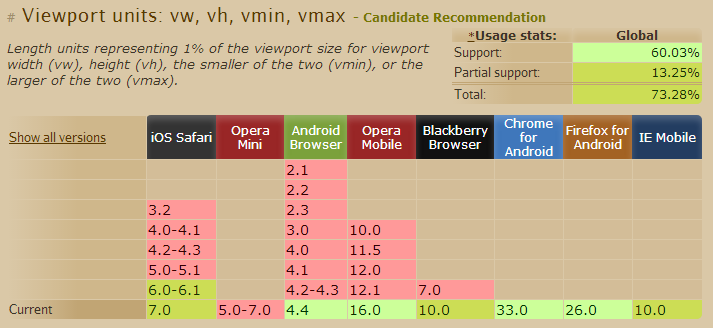
\includegraphics[width=1.0\textwidth]{viewport-units.png}
\end{figure}

In cases like this a developer can either limit their platform target range and make use of the fringe features available on mobile devices or use a polyfill also known as a shim. A polyfill is often referred to as code that substitutes the lack of a future API (application programming interface) by utilising existing features to mimic that of newer fully fledged implementations \cite{Lawson}. I my case I had to polyfill the lack of \textit{viewport units} in older mobile browsers. After searching for a solution I came across the slides of \cite{Kadrmas} presentation that detailed the use of \textit{em} units in HTML5 mobile games. \textit{em} units were originally intended for scaling document elements relative to the current font size. I used this to implement consistent scaling of my game across differing screen sizes by adjusting the root document element's font size relative to the screen width of the current device. This approach also made it easy to retain a specified aspect ratio, preventing any oddities when displaying on landscape displays.

% CONTINUE HERE

However, even when polyfilling potential feature gaps in browsers, issues can still occur under a variety of circumstances. One of the most reliable ways in which to ensure compatibility is to actually possess all the mobile devices you plan to support. This solution most of the time is impractical, especially if the developers fund are limit such as in my case. The next best alternative is to either emulator such devices or use online tools such as BrowserStack\footnotemark[4]. Figure \ref{browserstack} shows thumbnails of \textit{MindFlip} on \textit{Android} and \textit{iOS} browsers this is a helpful utility that assists in highlighting obvious incompatibility issues at a glance. The blank thumbnails quickly point out where my game is not loading, which allows me to select and prioritize what devices need debugging. However, with my limited workforce, budget, and time I could really only afford to debug devices I own such as the \textit{Samsung Galaxy S4} and the \textit{Google Nexus 7 (2012)}.

\footnotetext[4]{\url{http://www.browserstack.com/}}

\begin{figure}[h]{Screenshots of MindFlip on various mobile device browsers \label{browserstack}}
  \centering
    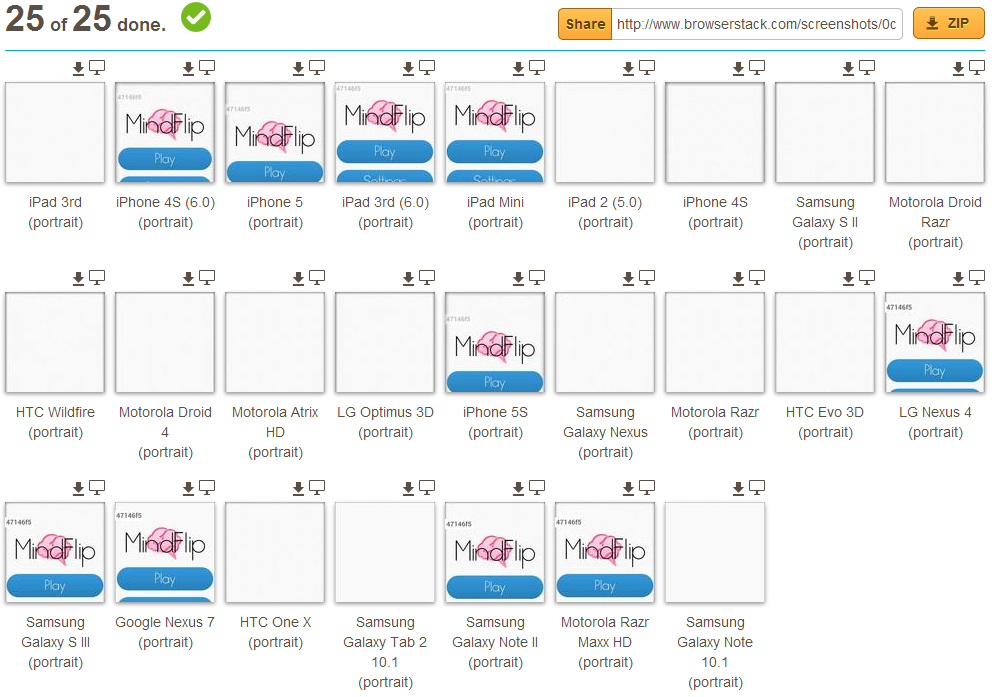
\includegraphics[width=0.8\textwidth]{browserstack.png}
\end{figure}

\section{Graphics}
When it comes to rendering in HTML5 are I many different options with varying advantages and disadvantages.

\subsection{Cascading Style Sheets (CSS)}
The fundamentals of web development are that the content of a website is typically marked down in a \texttt{.html} document and the style of this content is embedded alongside or defined within a \texttt{.css}. The browser parses the rules found in the stylesheet identifying referenced document elements in the process. This information then instructs the browser how to render the selected document elements often improving their otherwise bland presentation. Although \textit{HTML} has been getting a much needed update, this begs the question of what its companion \textit{CSS} has been doing in order to enhance the web experience. 

The latest iteration of \textit{CSS} often referred to as \textit{CSS3} provides new and interesting ways in which to style these elements. Notable features include rounded corners, shadows, gradients , transitions or animations , as well as new layouts like multi-columns , flexible box or grid layouts\footnotemark[5].

\footnotetext[5]{\url{https://developer.mozilla.org/en-US/docs/Web/CSS/CSS3}}

The support for these on mobile browsers has been around for quite awhile with much of the older versions supporting them through the use of vendor prefixes. These are a side effect of specification \textit{CSS3} still being a draft as such features were classified as experimental at the time. However, these are starting to be phased out as browser vendors start to agree on specifics and it also provides a means in which to use them providing legacy support for older browsers.

\subsection{Canvas}
\textit{Canvas} is probably the most significant feature that was introduced in \textit{HTML5}, especially for game developers. It finally enables developers to do interactive and dynamic graphics natively in the browser, without third-party plugins.

The new \texttt{<canvas>} element defines a graphics layer in a \textit{HTML} document that can be manipulated and drawn to through a \textit{JavaScript API}. Although this has been used in the context of desktop web applications to great effect it has suffered from performance issues on mobile browsers. This is often due to being limited to software rendering that only makes use of the device's \textit{CPU}. However, the performance of mobile devices has been increasing recent years with an emphasis on \textit{GPU} development \cite{Lin}. This has led to browser vendors adding support for \textit{GPU} accelerated rendering on mobile devices in places that use complex effects such as \textit{CSS3}.

However utilisation of these faster processors with the \textit{canvas} element has only just started to become common place. There are many ongoing software projects with a focus on accelerating the \textit{HTML5} canvas using the mobile device's \textit{GPU}. Unfortunately there is a lack of cross platform open-source projects that tackle this issue. \textit{Ejecta} is an is one such project but it current only supports \textit{iOS} and the hybrid mobile application framework \textit{Apache Cordova\footnotemark[6]} also provides an accelerated \textit{canvas} through a plugin called \textit{FastCanvas\footnotemark[7]}.

\footnotetext[6]{\url{https://cordova.apache.org/}}
\footnotetext[7]{\url{http://plugreg.com/plugin/phonegap/phonegap-plugin-fast-canvas}}

\subsection{WebGL}
\textit{WebGL} is a distillation of the popular \textit{OpenGL} making \textit{GPU} accelerated rendering in the browser now a reality. \textit{WebGL}, a \textit{JavaScript API} is based on the \textit{OpenGL ES (Embedded Systems)} subset, and as the name implies it was designed and optimized for embedded systems such as mobile devices. One streamlined modification \textit{OpenGL ES} made was the removal of the fixed-function \textit{API} introduced in \textit{OpenGL 1.0} enabling the use and compilation of modern shaders.

\textit{WebGL} has been in development for the past three years which came to maturity as of early last year when the first a stable version was released. As this is a new technology it has only just begun surfacing in the wild, one notable example is the \textit{PlayStation 4's} user interface. In a revealing presentation given by \cite{Olmstead} it was declared that the move to \textit{WebGL} was done to ensure cross platform support. This potentially hints at Sony's future plans to bring their games to multiple platforms including mobile devices through their \textit{PlayStation Now} streaming service.

However, the support for \textit{WebGL} through mobile browsers is essentially nonexistent to date. One company striving to change that is \textit{Ludei}, who are in the early stages of rolling out their new technology \textit{CocoonJS}. \textit{CocoonJS} is a means of packaging and publishing \textit{HTML5} applications on mobile devices. In amongst this framework is the facilitation of \textit{WebGL} letting it tap into the onboard \textit{GPU} available on most modern mobile devices. Many of the demos they provide demonstrate close to near native performance. This makes \textit{WebGL} a feasible avenue for game development on mobile devices, with the added bonus of being cross platform ready.

\section{Audio}
The state of \textit{HTML5} audio support in mobile browsers at this present time is still very limited and plagued with issues. Audio is a key component in delivering a satisfying game experience as it provides stimuli and feedback to the player. This can help further immerse the player in the game experience especially in main stream \textit{AAA} games. However, audio can play a part in mobile games too emphasising and cuing player interaction that would otherwise be difficult to prompt without the use of popups and explanatory text. These latter techniques are often avoided because they can bore and frustrate the player while breaking their immersion in the process. Audio can also serve as a brand mechanism for mobile games providing a strong theme that could be associated with good quality experiences.

Commonly the first action most players will take when playing a mobile games to instant mute or lower the audio. Players have a very low tolerance for disturbing sound design and due to earlier mobile games have been conditioned in this way. This stresses that audio must be used sparingly and in the appropriate context in order to deliver the full intended game experience \cite{Thomas}.

\subsection{\texttt{<audio>}}
The \texttt{<audio>} element is another significant addition from the \textit{HTML5} specification. It provides developers a way to define sound content within a \textit{HTML} document which can then be loaded and played back by web browser. Because of this element web applications can now finally deliver an audio experience that before was impossible to achieve without the use of a third-party plugin.

Support for this element in mobile browsers is widespread however there are many discrepancies between them. Here is a list of some of the known issues that currently effect mobile browsers taken from \textit{caniuse.com\footnotemark[8]}.

\footnotetext[8]{\url{http://caniuse.com/\#feat=audio}}

\begin{itemize}
  \item Audio played from the element in iOS always plays in a full screen player.
  \item Playback rate not supported on the stock android browser.
  \item Only one Audio file can be played at one time in iOS and Android browsers which forces you to use sprites for multiple audios.
  \item Audio in iOS can not be auto played. It even starts downloading after a user triggered event.
  \item Volume is read-only on iOS.
\end{itemize}

Much of these restrictions imposed by mobile web browsers make it awkward to utilise \texttt{<audio>} as an competent solution for dynamic sound effects and background music. This also poses a problem when trying to compete with native mobile games as features such as multichannel audio and equalizers come standard with their relative \textit{SDK}.

\subsection{Web Audio API}
The Web Audio API is an experimental high-level \textit{JavaScript API} that is currently being drafted and developed by \textit{Google} and the \textit{W3C\footnotemark[9]}. This \textit{API} provides richer methods to manipulate and generate audio through signal processing and synthesis. This also includes the ability to load and playback audio files similar to the \texttt{<audio>} element. A similarly the \textit{MediaStream API\footnotemark[10]} developed by \textit{Mozilla} is trying to achieve the same functionality focusing on the streaming of both audio and video related data.

\footnotetext[9]{\url{http://www.w3.org/TR/webaudio/}}
\footnotetext[10]{\url{https://developer.mozilla.org/en-US/docs/WebRTC/MediaStream_API}}

This definitely appears to be a more appropriate technology for the implementation of game related audio. However, these technologies are much newer than the \texttt{<audio>} element and have yet to be implemented in any of the stock mobile browsers with the exception of \textit{iOS Safari} versions \texttt{6.0-7.0\footnotemark[11]}.

\footnotetext[11]{\url{http://caniuse.com/\#feat=audio-api}}

\subsection{Native Audio}
With the advent of hybrid mobile applications frameworks in some cases it is now viable to bridge to the mobile operating system's native media player. This presents much fewer headaches to developers as these \textit{APIs} have been around for much longer and are therefore adequately stable.

In my project I used \textit{Apache Cordova} which has a official plugin that bridges the gap from \textit{JavaScript} to most naive mobile media players. This allowed me to make calls to the \textit{Media} plugin's \textit{API} and have the native media player load and playback audio files that were in my web applications directory. Unfortunately I found \textit{Apache Cordova's} official \textit{Media} plugin had quite high latency which detracted from the tactile feel I was trying to achieve. After researching I found a custom \textit{LowLatencyAudio} plugin that had been developed by \citep{Trice} for the \textit{PhoneGap} framework (the predecessor to \textit{Apache Cordova}). This has plugin was since ported to \textit{Apache Cordova} by \citep{Xie} for \textit{Android} and \textit{iOS} which I utilised in my project.

\section{Game Design}
a

\subsection{Player Interaction}
a

\subsection{Gameplay \& Mechanics}
a

\subsection{Feedback}
Throughout the development and prototyping of MindFlip it was important to take into consideration the reactions and feedback of players. So whenever the chance arose I would hand over my phone containing my latest stable build of the game and observe others playing it from a third-party perspective.

Preconceptions can be a double edged sword when used in game design. Often they can be used to draw parallels between activities in contemporary games such as my own. This acts as a shortcut when teaching a player new or similar gameplay mechanics. However, these can also be stumbled upon accidently from a developer's perspective as their own preconceptions about games will likely be vast by comparison to the average player.

This was the case with the initial draft of introductory level. In the beginning the first two card symbols the player encountered were a red nought and a blue cross on a three-by-three grid. After showing the game to my sister while providing no tutorial, the first actions she made were to produce a winning \emph{Tic-tac-toe} game state. This made it apparent that there was a flaw in my game design, because the symbols are common to a pre-existing game namely \emph{Tic-tac-toe} the player receives mixed signals about how to play the game from the offset leading to frustration and confusion. I later decided to go for simpler more abstract symbols such as circles, squares, and triangles in my initial set of levels do to their generic associations they imply simplicity leaving the player open to learn the game mechanics.

\section{Development Stack}
When creating a game targeting HTML5 it can be difficult to know what workflow to invest in. Developers each have their own preferences and beliefs as to what is the best way to work with their priorities often being similar but achieved in different ways.

\subsection{Preprocessors \& Alternatives}
\textit{JavaScript} in its current state (\textit{ECMAScript 5.1}) is an underwhelming language, especially when compared to more mature languages such as \textit{C++} or \textit{Java}. It lacks native support for object-orientated features such as inheritance, generics, and abstraction. Originally \textit{JavaScript} was never intended for use in large-scale development projects however, due to its inherent portability it has become widespread. Until its apparent deficiencies are rectified and standardised in its next iteration (\textit{ECMAScript 6}), developers have to over utilise its strengths, such as being loosely typed. To help aleve \textit{JavaScript's} growing pains many organisations have been developing alternatives and middle ware to deal with its short comings.

Heavily standardised languages such as \textit{JavaScript} often have very long iteration cycles, making it difficult for them to adapt swiftly however, this does help to ensure and maintain a language's stability in the long term. By comparison \textit{transpilers} (source-to-source compilers) can transform a better suited custom language into plain \textit{JavaScript}, by shimming the missing functionality at compile time. They also make it easier for developers to transition to web development without having to learn the semantics of \textit{JavaScript}. In figure \ref{ranking} are the top thirty-nine most popular programming languages as of January 2014. These statistics were calculated based upon their frequency of occurrence on GitHub (x-axis) and Stack Overflow (y-axis); popular community websites with a focus on programming. By comparing it to one from last year\footnotemark[12] it is clear to see their has been a rise in popularity. Some such preprocessors include CoffeeScript\footnotemark[13], Clojure\footnotemark[14], Dart\footnotemark[15] and TypeScript\footnotemark[16]. The full graph\footnotemark[17] is cumbersome so this snippet is only of the top quadrant.

\footnotetext[12]{http://redmonk.com/sogrady/2013/07/25/language-rankings-6-13/}
\footnotetext[13]{http://coffeescript.org/}
\footnotetext[14]{http://clojure.org/}
\footnotetext[15]{https://www.dartlang.org/}
\footnotetext[16]{http://www.typescriptlang.org/}
\footnotetext[17]{http://redmonk.com/sogrady/2014/01/22/language-rankings-1-14/}

\begin{figure}[h]{The RedMonk Programming Language Rankings: January 2014 \label{ranking}}
  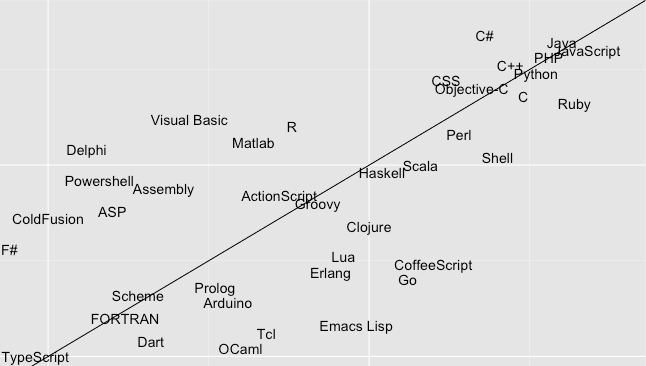
\includegraphics[width=1.0\textwidth]{lang-rank-114-wm.png}
\end{figure}

The advantages of transpilers often mean that less can be written in order to achieve the same functionality in its targeted language. Simple common activities such as array iteration, class extension, and appending vendor prefixes can become unnecessarily ceremonious especially in the case of \textit{JavaScript} when shimming non-existent functionality. These transpilers can offer an alternative means in which to achieve the same results with less code and effort required on the part of the developer.
\subsubsection{Dart}
\textit{Google's Dart} ``is a new platform for scalable web app engineering'' which comes in the form of several tools. First there is \textit{Dart} the language which is an alternative to writing plain \textit{JavaScript} with a host of additional built-in and libraries language features akin to \textit{Java} \cite{Fortuna}. Second there is \textit{DartVM} a virtual machine that comes as a standalone program and also happens to be embedded in the \textit{Google Chrome} browser. The \textit{DartVM} works similarly to a typical \textit{JavaScript} virtual machine with the difference being it interprets \texttt{.dart} code instead of \textit{.js} with significant performance advantages \cite{Schneider}. Lastly there is the \textit{dart2js} compiler, which is effectively a backwards compatibility tool to ensure any application created on the \textit{Dart} platform will still work through conventional means.

\subsubsection{TypeScript}
\textit{Microsoft's TypeScript} by its own admission ``is a typed superset of JavaScript that compiles to plain JavaScript.'' which makes it very flexible alternative. This effectively means that you can continue to write plain \textit{JavaScript} and no restrictions will be imposed by the \textit{TypeScript} transpiler. This helps greatly if a developer already has a large \textit{JavaScript} codebase which they wants to utilise during the development of a large scale application. \textit{TypeScript} offers some of the inherently missing language features of \textit{JavaScript} such as type annotations, classes, interfaces and modules. There are also plans to support \textit{ECMAScript 6} features once it becomes the standard. Another positive remark about the output produced by the \textit{TypeScript} transpiler is it produces rather legible \textit{JavaScript} making it easy to see the relationships between the source and target languages.

Because the compile target of these transpilers is \textit{JavaScript} it is possible to take advantage of them when developing mobile web applications such as video games. When I first started developing my game I chose to use \textit{TypeScript} because it was syntaxitcally similar to that of \textit{ActionScript 3}, where my background lies. However, due to the immaturity of the project at the time and a lack of core \textit{JavaScript} knowledge on my part, I felt it was best not to continue using it as I did not have the time to invest in fully learning its ins and outs. I also felt working at this level of abstraction could potentially lead to delays when debugging later in development. However, as of the 2nd of April 2014 close to the time of writing the specification for \textit{TypeScript 1.0} has been finalised and its current status is \textit{stable}. Going forward after this project I am eager to re-evaluate it now that it has had time to mature.

\subsection{JavaScript Modules}
\textit{JavaScript} is typically created as separate \texttt{.js} text files that are then referenced in a \texttt{.html} document by \texttt{<script>} tags. When the web browser finds scripts linked by these tags it will request them from the web server and inject them into the document once loaded. This presents a few problems for large and complex web applications which will often require many scripts each having to be requested and loaded synchronously. Every one of these request has an overhead, which is compounded when a vast quantity are being made. This can lead to suboptimal load times.

To combat this problem a developer could attempt to write all their code in one \texttt{.js} file. This file can quickly become colossal making it difficult to manage and refactor, especially on large scale projects. Alternatively the developer can split their code into several \texttt{.js} files that will all have to be referenced by a corresponding \texttt{<script>} tag. Therefore the more organised the codebase becomes the more requests the browser has to make. The developer also has to micromanage these \texttt{<script>} tags to ensure their ordering is correct. The ordering is important because one script could be referencing another that has not yet been loaded, thus causing runtime errors. This approach also presents issues when attempting to introduce software engineering best practices such as unit testing because the interdependencies between these scripts are not clearly defined.

One solution to this common problem is the \textit{module} design pattern. \textit{JavaScript} has an official name \textit{ECMAScript}, and version \textit{5.1} (ECMA-262\footnotemark[18]) is the current standard. However, this present language specification does not support \textit{modules}. The 6th version\footnotemark[19] of the \textit{ECMAScript} specification is currently being drafted with plans to include modules but until then developers must seek other alternatives.

\footnotetext[18]{\url{http://www.ecma-international.org/ecma-262/5.1/}}
\footnotetext[19]{\url{https://people.mozilla.org/~jorendorff/es6-draft.html}}

There are a variety of libraries that offer solutions such as \textit{RequireJS\footnotemark[20]}, \textit{HeadJS\footnotemark[21]} and \textit{yepnope.js\footnotemark[22]}. However, personally I found \textit{Browserify\footnotemark[23]} to be the simplest and the most supported amongst the \textit{Node.js} community. \textit{Browserify} enables developers to write their \textit{JavaScript} code in numerous files and when one file requires another it can be injected via the \texttt{require(`example');} function. Once a developer has written all their code they can recursively bundle all their modules starting with a root module similar to that of a main class in conventional programming languages. This provides the developer with the best of both scenarios as all their code will be built into a single \texttt{.js} file (including their external libraries), while allowing for easy management and refactoring of their core codebase through individual source files.


\footnotetext[20]{\url{http://requirejs.org/}}
\footnotetext[21]{\url{http://headjs.com/}}
\footnotetext[22]{\url{http://yepnopejs.com/}}
\footnotetext[23]{\url{http://browserify.org/}}

Most might think that this will in turn cause complications when debugging. As when the code breaks it will do so in the colossal \texttt{.js} file that the browser is running. This is where source maps come in. Source maps provide linkage between the original \texttt{.js} source files and their bundled counterparts making breakpoints and stepping through code painless. \cite{Seddon}

This process can also be made seamless by \textit{Watchify} which automatically recompiles the \textit{Browserify} bundle whenever a module file has been updated. This allows for the developer to work on their original source files and as soon as the file has been saved it have rebuilt the bundle ready to reloaded in the browser for testing.

After the modules have been bundled a further step called minification which involves taking legible \textit{JavaScript} and compressing it down into its most minimal form by removing unnecessary characters such as a whitespace and shrinking instance names. This process can further decrease the \texttt{.js} file size making load times marginally faster while also partially obfuscating the original code from prying eyes.

\cite{Hanselman} proclaimed that \textit{JavaScript} has become akin to a assembly language for the web. Which is the impression a lot of people will get when taking a peek at the source of popular website such as \textit{Google} or \textit{Facebook}. This is some what understandable given the that \textit{JavaScript} is as low-level as developers can get when programming for the web. However, a happy side effect of being closely tide with the web is it has become now one of the most portable languages to date, because every web enabled device has a browser, and every browser has a \textit{JavaScript} virtual machine. This makes \textit{JavaScript} a very cross-platform language to develop games with and reaching a wide audience is key when maximising chances for success.

\subsection{Model View * (MV*)}
To keep my project structure and programming semantics organised I wanted to employed the use the MVC (model view controller) design pattern in development. However, because of the inherent structure of web applications a controller often is not a ``true'' controller and mislabelled which has led to the term MV* framework implying a substitution of the controller with a more appropriate alternative. I had begun development initially using TypeScript later moving to plain JavaScript but I found my inexperience with the language rapidly led to jumbled spaghetti code. I felt that the use of a MV* framework would assist me retaining a legible codebase.  Which became imperative when frequently switching between other coursework projects that also required prolonged development in differing programming languages.

As with most JavaScript frameworks there are countless variants on offer which made it daunting to select one. It was important to make a firm decision as limiting time constraints prevented me from investing time in learning the pros and cons of each. TodoMVC\footnotemark[25] is a project with the intent of assisting developers select a JavaScript MV* framework. TodoMVC provides developers with a simple todo web application constructed with each of these varying MV* frameworks, allowing them to quickly browser the source code of each and determine whether it suits their needs.

\footnotetext[25]{\url{http://todomvc.com/}}

I quickly came to the decision of Backbone.js\footnotemark[26] because of its flexibility, large community following, and modular design. As described in a presentation given by \citet{Bull} Backbone.js is the equivalent of a \textit{knife/spoon/fork} on a camping trip. Which I interpreted as modular implying that there is no imposed exclusivity between its internal components. This allowed me to gradually implement the use of its Model, View, Collection, and Router classes throughout my development process not forcing me to learn everything at once but only when I required it.

\footnotetext[26]{\url{http://backbonejs.org/}}

\subsection{Templates}
a


\subsection{Text Editors \& IDEs)
During this project I also assessed a various tools and applications I could utilise in my development work flow. The most fundamental tool required is that of a text editors and/or IDE (integrated development environment). They help to maximise the output of a developer by offering efficient procedures such as autocompletion, refactoring and build automation. In this section I will be presenting the solutions I explored which boosted my productivity.

\subsubsection{Adobe Brackets}
Brackets\footnotemark[27] is an open source code editor for web designers and front-end developers constructed with HTML, CSS and JS and maintained by Adobe. It has a comprehensive suite of plugins\footnotemark[28] providing developers a great way to customise it to suit their needs. As the project is open source it allows developers to create and submit their own plugins if their niche has yet to be filled. One of the most useful features I found myself taking great advantage of is the live preview mode letting me type code while viewing its results instantaneously in the browser. When tweaking the aesthetics of my game I could change colours and styles rapidly making decision based upon the live preview as to whether they were appropriate. The nested nature of this editor being built with the languages it is providing the means to edit also benefits from the inherent portability of these languages making it avaliable cross platform on Windows, Linux and OSX.

\footnotetext[27]{\url{http://brackets.io/}}
\footnotetext[28]{\url{https://brackets-registry.aboutweb.com/}}

\subsubsection{Sublime Text}

\subsubsection{Visual Studio 2013}
\subsubsection{WebStorm}

\section{Mobile Deployment}
One of the challenges that faces mobile developers is how to package their applications for the mobile platform, which spans such a wide variety of hardware and operating systems (iOS\footnotemark[29], Android\footnotemark[30], Windows Phone\footnotemark[31], Ubuntu\footnotemark[32]). This poses a problem especially for the smaller companies as to develop native variants of an application for each platform while retaining a common vision is demanding on both financial and chronological frontiers. Larger companies that facilitate and accommodate such resources, can however frequently benefit from more seamless experience. Most native applications built with their corresponding software development kits (SDKs) which have direct access to device specific application programming intefaces (APIs). This often results in native applications having faster performance and better system user interface integration. Native applications compile to binary machine code that is then interpreted via its relative hardware architecture making it vastly faster than JavaScript which is interpreted at run-time via a browser or web-view. This is most apparent when it comes to developing 3D gaming experiences as these can often be most the most performance taxing, \cite{Kulloli}.

\footnotetext[29]{\url{http://www.apple.com/ios/}}
\footnotetext[30]{\url{http://www.android.com/}}
\footnotetext[31]{\url{http://www.windowsphone.com/}}
\footnotetext[32]{\url{http://www.ubuntu.com/phone}}

When comparing HTML5 based mobile applications to native there was another significant disadvantage as there was no way to access device APIs. Such APIs are required to make use of the most hardware features on mobile devices such as the camera, device orientation and battery status. Especially considering that each API varies dependant on operating system and then again on hardware specification. For instance not all mobiles have front facing cameras or high-dpi (dots per inch) screens but a vast majority do. So it becomes quite a challenge when trying to build an application that adapts from phone-to-phone without excluding a particular sector of an audience from the core user experience, \cite{Charland}.

A project with the sole purpose of remedying such issues is that of PhoneGap a mobile development framework originally created by a company called Nitboi. After PhoneGap began to make strides the company was purchased and enveloped by Adobe in 2011, \cite{Adobe}. Then after the project matured under Adobe's supervision the project was donated to the Apache Software Foundation. This was to ensure that the project was properly maintained when made open source under the Apache License Version 2.0\footnotemark[33]. A formality due to this hand over was that the open source variety of the project had to operate under a different name to avoid trademark ambiguity, \cite{Leroux}. Adobe's PhoneGap still functions as a separate entity as a distribution of Apache Cordova offering services such as cloud compilation\footnotemark[34].

\footnotetext[33]{\url{http://www.apache.org/licenses/LICENSE-2.0.html}}
\footnotetext[34]{\url{https://build.phonegap.com/}}

Apache Cordova\footnotemark[35] is a platform for building native mobile applications using HTML, CSS and JavaScript. It achieves this by providing developers with a set of relative device APIs that allow for access of functions previous obfuscated from web technologies by the native system. It also assists with handling a lot of the cross-platform concerns previously mention when targeting multiple platforms and device hardware.

\footnotetext[35]{\url{http://cordova.apache.org/}}

\subsection{Packaging}
\textit{\texttt{eck!}}

\subsection{Debugging}
It took me awhile to finally settle upon the debugging solution of my development stack and I tried a few approaches with varying success. It was important to be able to quickly prototype on my desktop computer as well as my mobile devices. On desktop computers this is relatively easy as most desktop browsers applications have built in development tools with a variety of features. However, understandable this is not the case commonly on mobile browsers as screen space is limited and it would be difficult to convey the vast streams of data are under the hood of a typical web application. Even the bare minimum tools such as a console are often absent in mobile browsers which are a necessity when trying to diagnose runtime errors in generated by JavaScript as well as reading the output \texttt{console.log()}.

\subsubsection{Apache Ripple}
Apache Ripple\footnotemark[36] is a companion project of Cordova consists of a web based mobile environment simulator design to emulate the conditions of a packaged Cordova application. It has options for manipulating mobile specific features such as GPS (global positioning system) geolocation and device orientation. This can be useful for developers when rapidly prototyping an application that makes use such mobile specific features. This solution was used for a while until the lack of up-to-date documentation and dwindling support hampered progress during early development.

\footnotetext[36]{\url{http://ripple.incubator.apache.org/}}

\subsubsection{Weinre}
Weinre\footnotemar[37]k (web inspector remote) is a debugger application created by Patrick Mueller\footnotemark[38] who is also a contributor to the Apache Cordova project. This application works similar to the built-in desktop browser debuggers and inspectors with the added bonus of having a remote target. By including a remote JavaScript file hosted on a local weinre server the mobile device can be linked letting it send and receive debugger data from the server. This lets developers inspect and manipulate the mobile devices web browser. The key issue that prevented the further use of this application in the project's development was that in combination with Apache Cordova it was not able to log any information before the script was loaded and the console was initialized. So when it came to analysing the initial portion of an application's lifecycle the data generated was restricted by this dependency.

\footnotetext[37]{\url{http://people.apache.org/~pmuellr/weinre/docs/latest/Home.html}}
\footnotetext[38]{\url{http://muellerware.org/}}

\subsubsection{Adobe Edge Inspect}
Adobe Edge Inspect\footnotemark[39] previously known as Adobe Shadow is a tool built on top of Weinre that lets developers preview and inspect across multiple devices concurrently. 
When it was being assessed for use in this project's development the free version was limited to testing on one device, since then it has become exclusively a paid product. Another disadvantage that came with using this solution is the web application had to be viewed through their Adobe Edge mobile application similar to that of a browser. This made it impossible to debug the game through its targeted environment bundled within a Cordova application.

\footnotetext[39]{\url{http://html.adobe.com/edge/inspect/}}

\subsubsection{Chrome DevTools}
Chrome DevTools\footnotemark[40] was definitely the most comprehensive and painless solution discovered during development. DevTools encapsulates mobile emulation\footnotemark[41] as well as remote debugging\footnotemark[42] of Android's WebView on versions 4.0 and above which Cordova uses to display the embedded web content. During development some of these features were classified as ``experimental'' but still accessible through Chrome Canary\footnotemark[43], a custom variant of Google's browser designed for developers and early adopters of fringe web technologies. DevTools provided a quick and effective way to iteratively test the game first on the desktop platform, a mobile emulation, and finally when deployed on mobile devices.

\footnotetext[40]{\url{https://developers.google.com/chrome-developer-tools/}}
\footnotetext[41]{\url{https://developers.google.com/chrome-developer-tools/docs/mobile-emulation}}
\footnotetext[42]{\url{https://developers.google.com/chrome-developer-tools/docs/remote-debugging}}
\footnotetext[43]{\url{https://www.google.co.uk/intl/en/chrome/browser/canary.html}}


\clearpage
\bibliography{5939968}

\end{document}

